\FloatBarrier
\noindent Using the boosted decision trees with the AdaBoost method, we grow our decision tree using the first 8 predictors, that is, we did not train the tree on the frequencies of the five test words. We use 50\% of the data to grow the tree, and use the remaining data for testing. The resulting separation of the test data by the decision tree is shown in figure \ref{fig:AdaBoost8}. The accuracy of the decision tree is 63.4\%.
%\begin{figure}[h]
%\centering
%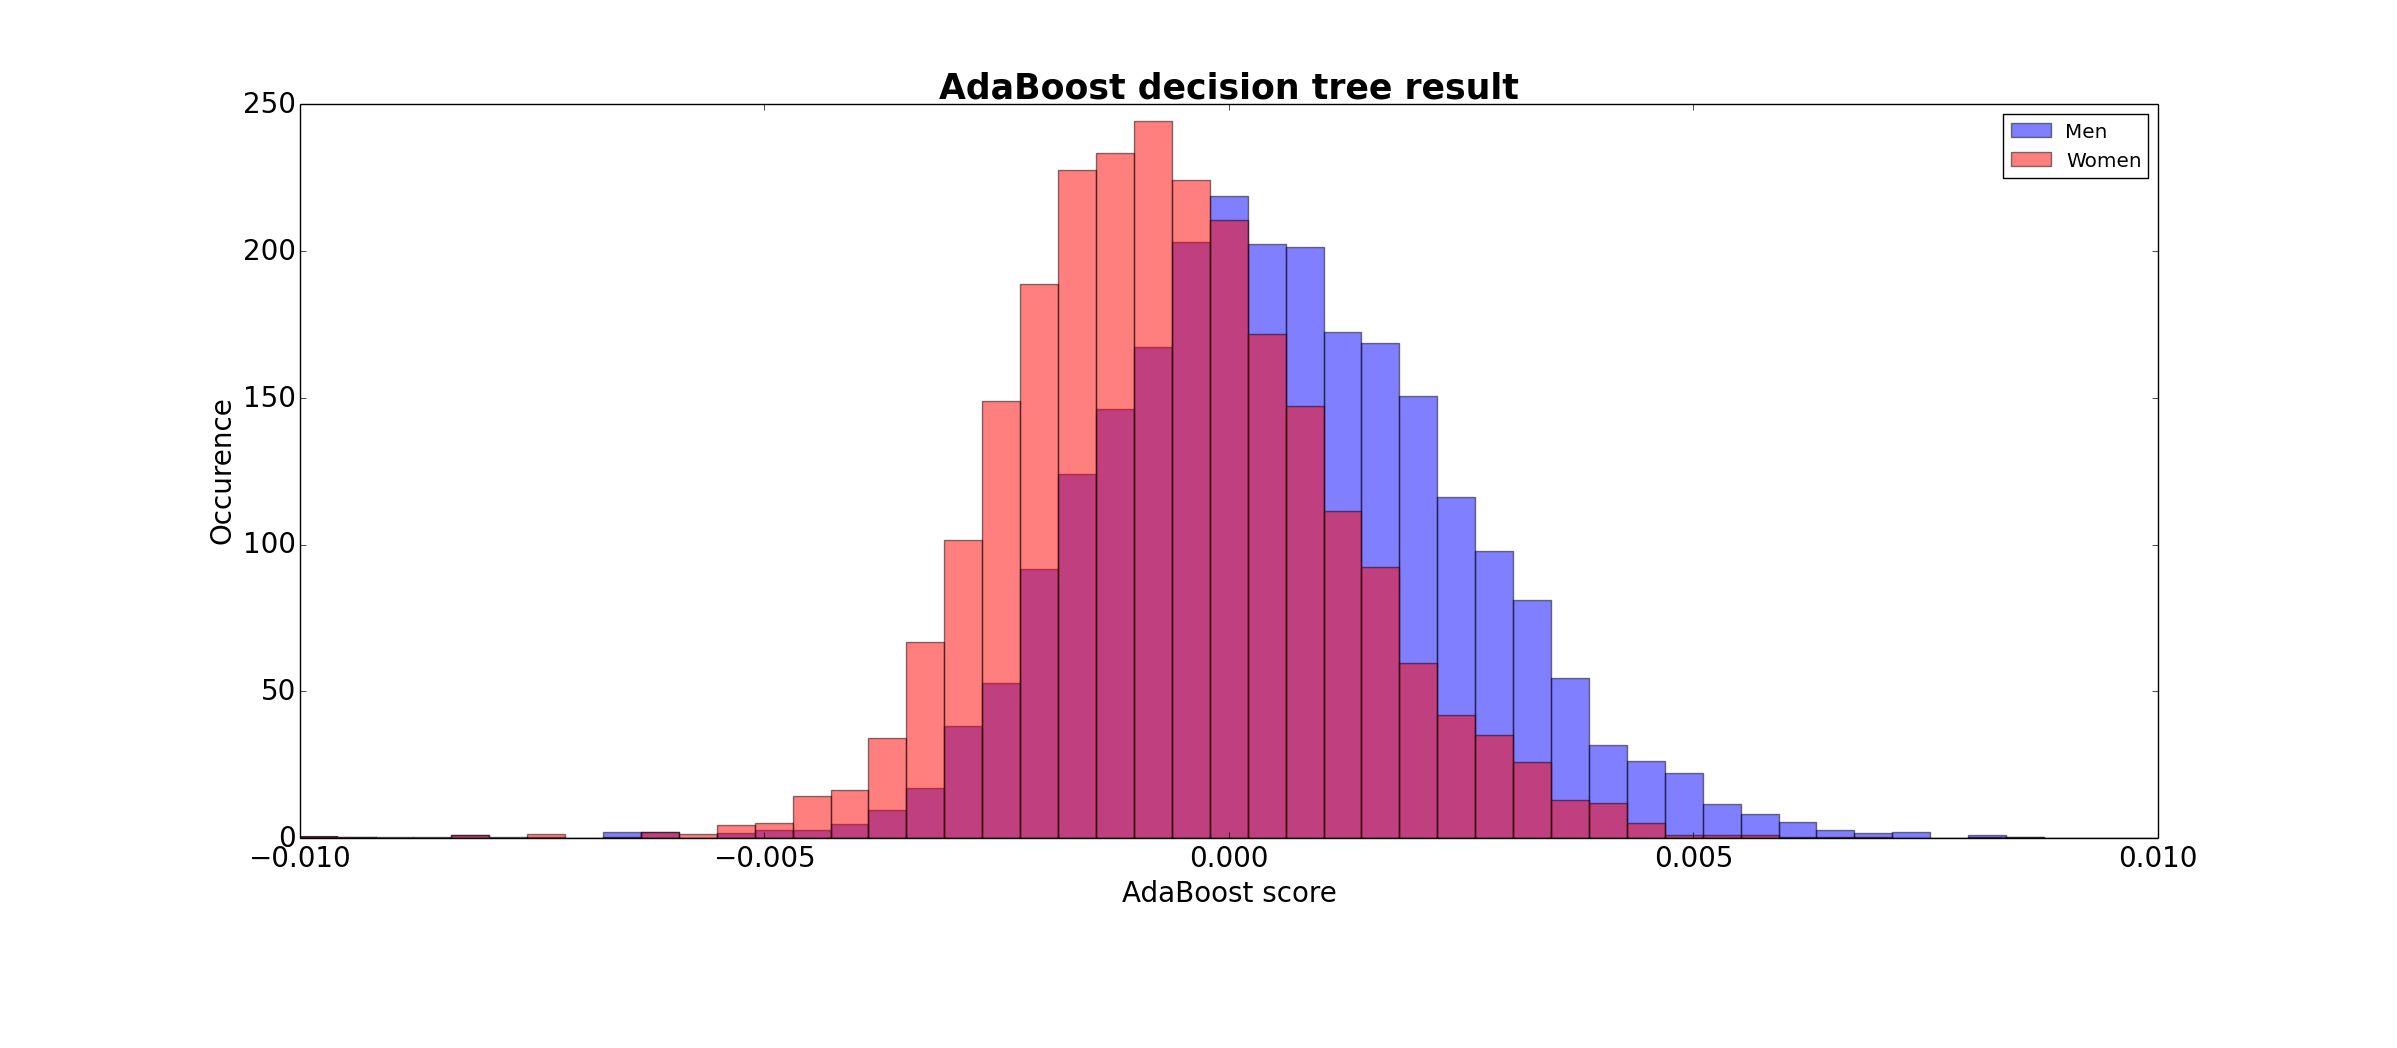
\includegraphics[width=\textwidth]{Pix/HistAdaB8.png}
%\caption{The separation of the test data using the AdaBoost method and predictors 1-8. The tree is grown using 50\% of the data set and remaining 50\% is the test data. A value smaller (larger) than zero corresponds to the label "female" ("male")}
%\label{fig:AdaBoost}
%\end{figure}

\noindent We also run the algorithm using all 13 predictors, and agian we use 50\% of the data to grow the tree. The results using these predictors is shown in figure \ref{fig:AdaBoostAll}. The accuracy of the decision tree is here 65.8\%.\\
%\begin{figure}[h]
%\centering
%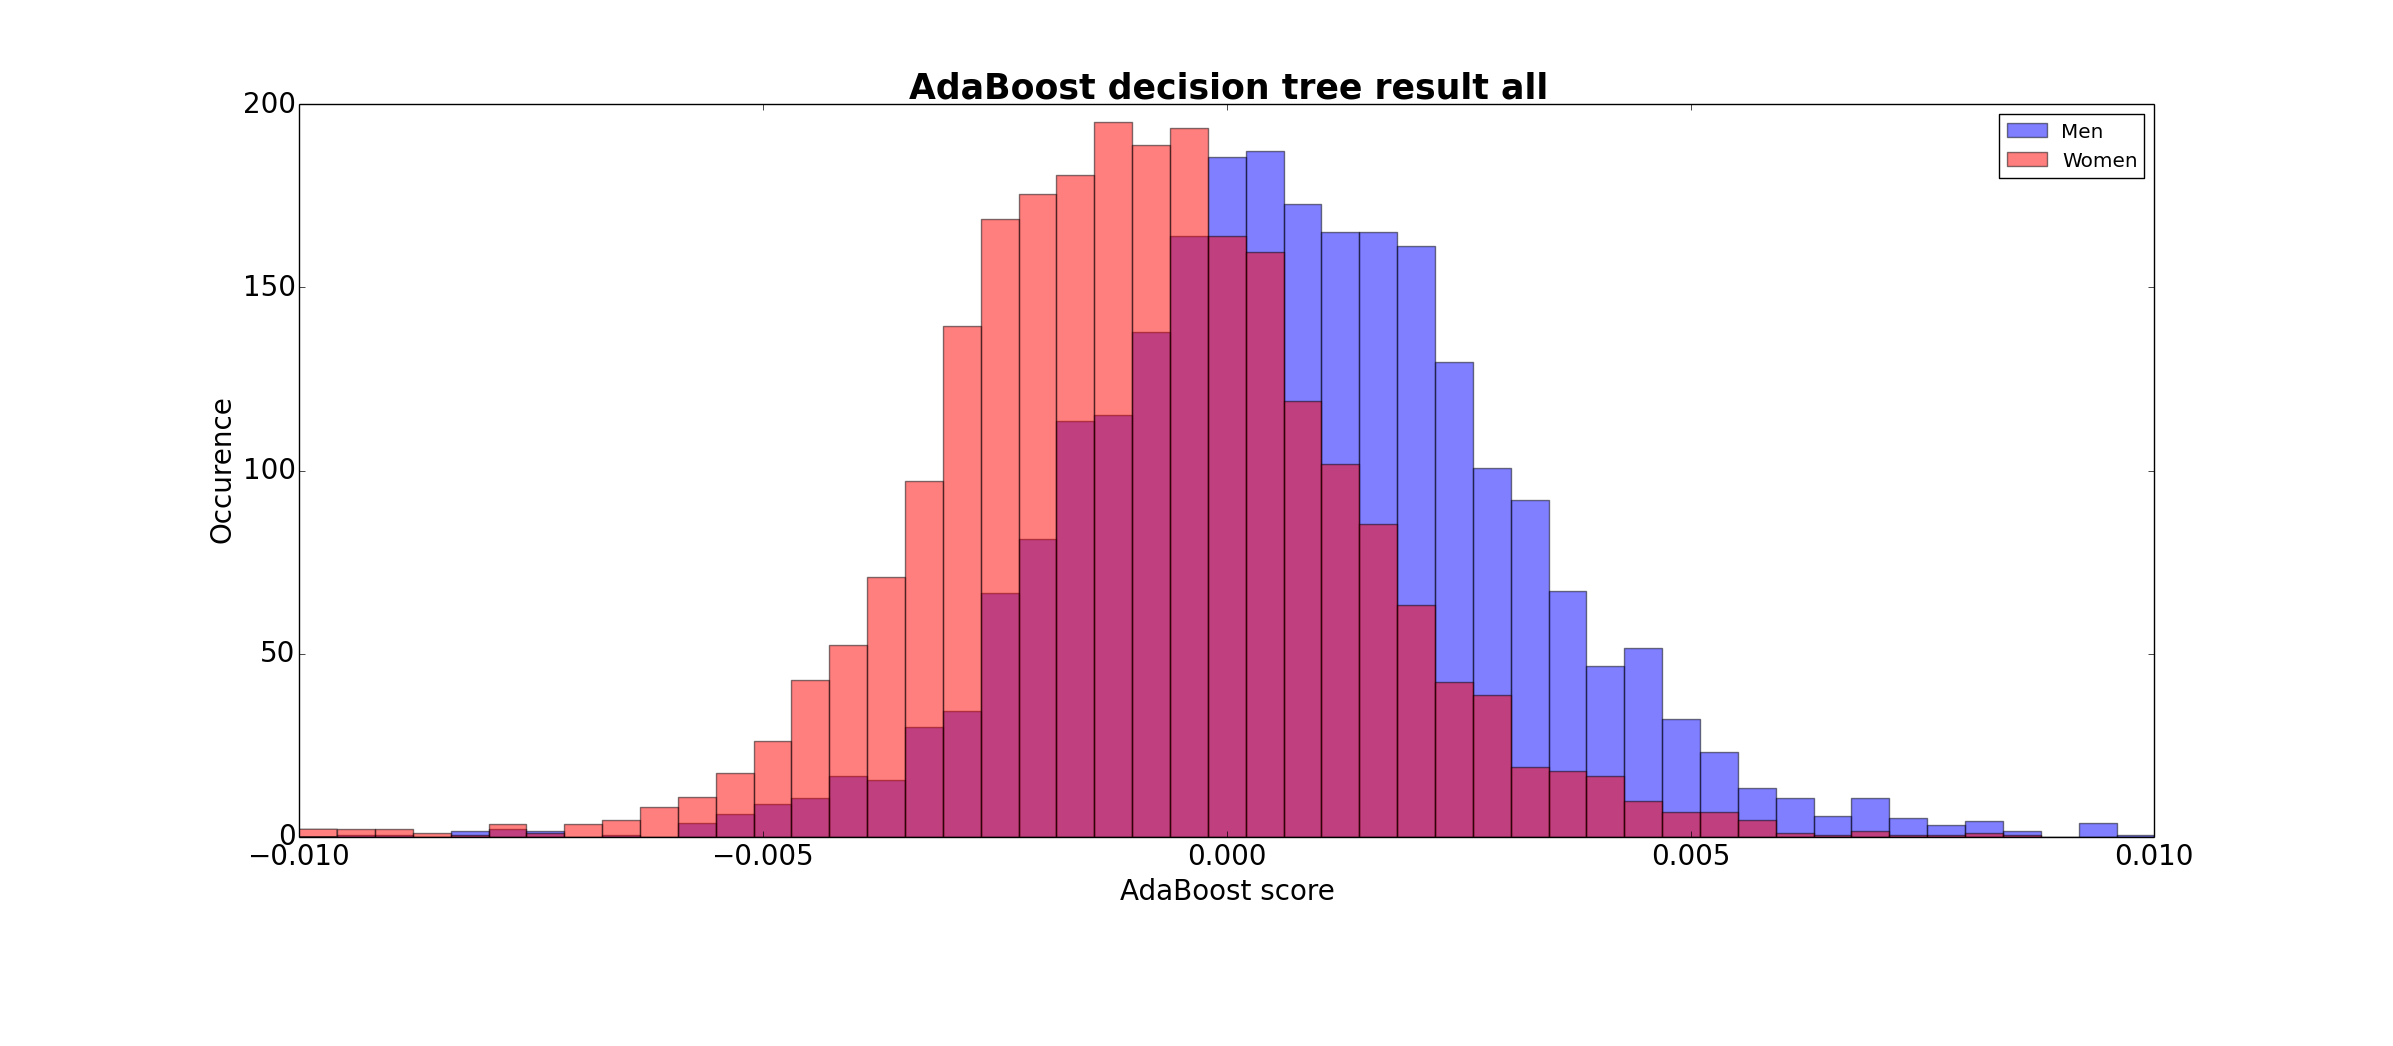
\includegraphics[width=\textwidth]{Pix/HIstAdaAll.png}
%\caption{The separation of the test data using the AdaBoost method and predictors 1-13. The tree is grown using 50\% of the data set and remaining 50\% is the test data. A value smaller (larger) than zero corresponds to the label "female" ("male")}
%\label{fig:AdaBoostAll}
%\end{figure}

\begin{figure}[h]
    \centering
    \begin{subfigure}[b]{0.45\textwidth}
        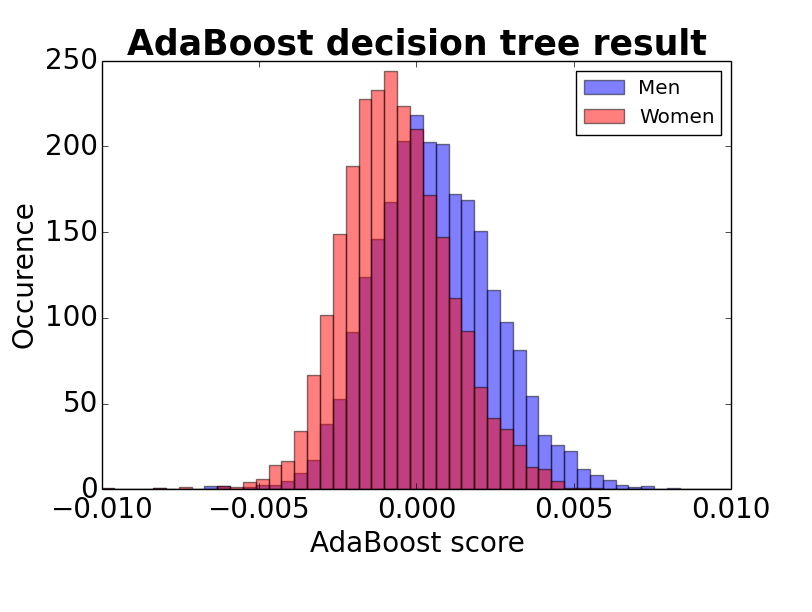
\includegraphics[width=\textwidth]{Pix/HistAdaB82.png}
		\caption{The separation of the test data using the AdaBoost method and predictors 1-8.}
		\label{fig:AdaBoost8}
    \end{subfigure}
    ~
    \begin{subfigure}[b]{0.45\textwidth}
		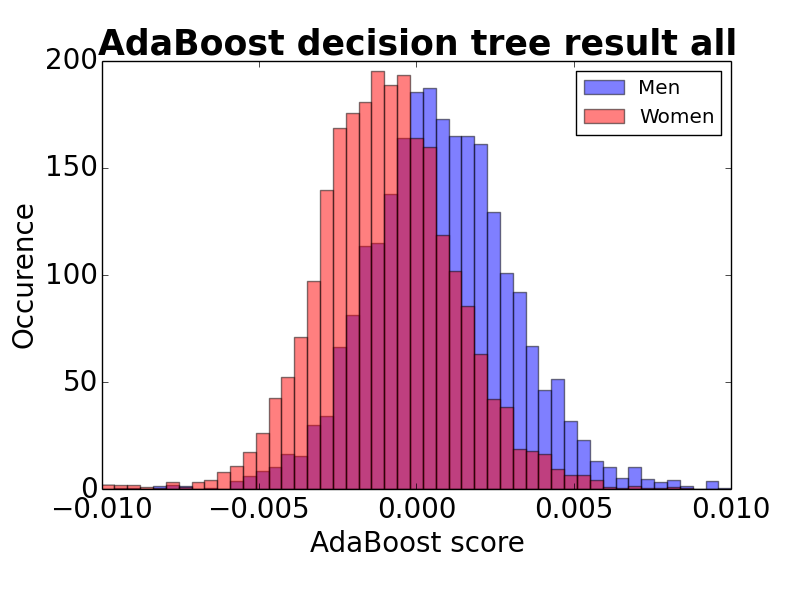
\includegraphics[width=\textwidth]{Pix/HIstAdaAll2.png}
		\caption{The separation of the test data using the AdaBoost method and predictors 1-13.}
		\label{fig:AdaBoostAll}
    \end{subfigure}
    \caption{The tree is grown using 50\% of the data set and remaining 50\% is the test data. A value smaller (larger) than zero corresponds to the label "female" ("male"). The colors of the two histogram corresponds to the true label.}
	\label{fig:AdaBoost}
\end{figure}

\noindent For this project we also trained a SVM for comparison with the AdaBoost method. Here we used  predictors 1-8.
With these 8 predictors, we train the SVM on 20\% of the data, and use the remaining 80\% of the data as test data. The accuracy of the algorithm on the test data is 62.4\%.

\noindent We train the SVM again, now using 50\% of the data as training data. The increase in training data does not improve the performance significantly, as the accuracy on the test data is now 63.4\%.

\noindent The 5-fold cross-validation error on the training sample is shown in figure \ref{fig:SVM_Train}.

\begin{figure}[h]
    \centering
    \begin{subfigure}[b]{0.45\textwidth}
        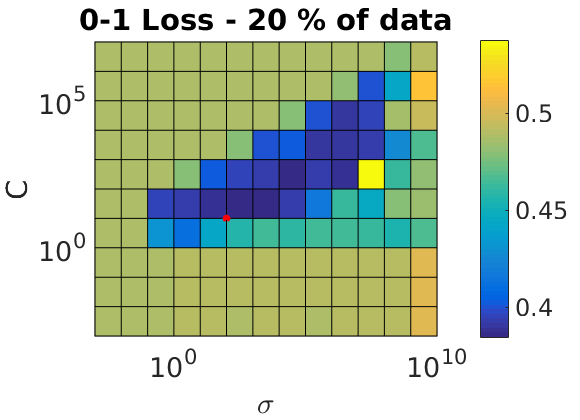
\includegraphics[width=\textwidth]{Pix/SVM_02.png}
		\caption{Using 20\% of the data as training data. Minimum loss found is 0.362}
		\label{fig:SVM_02}
    \end{subfigure}
    ~
    \begin{subfigure}[b]{0.45\textwidth}
        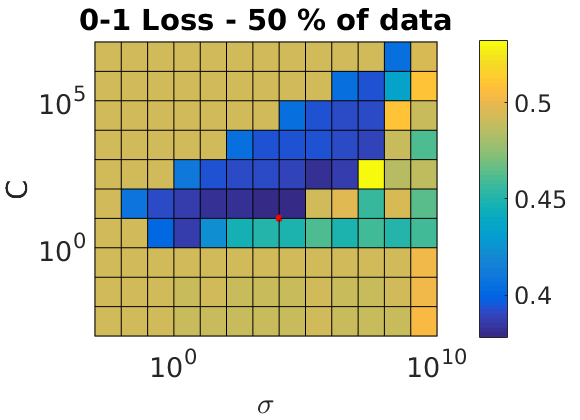
\includegraphics[width=\textwidth]{Pix/SVM_05.png}
		\caption{Using 50\% of the data as training data. Minimum loss found is 0.350}
		\label{fig:SVM_05}
    \end{subfigure}
    \caption{The five-fold cross-validation loss of the SVM as a function of the parameters $C$ and $\sigma$. The red point shows the minimum loss, and the corresponding values of the parameters are used for the final SVM}
	\label{fig:SVM_Train}
\end{figure}

\noindent The scores of the test data generated by the SVM is shown in figure \ref{fig:SVM_Result}.

\begin{figure}[h]
    \centering
    \begin{subfigure}[b]{0.45\textwidth}
        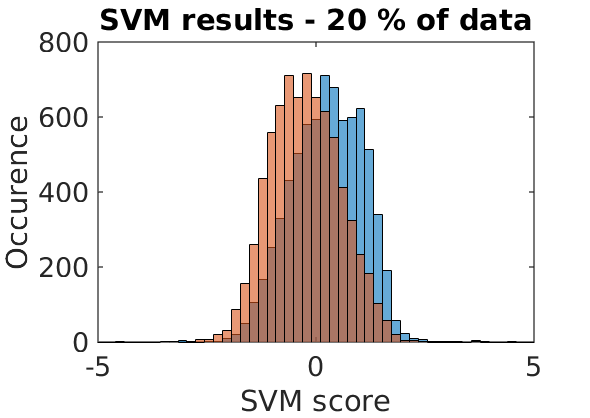
\includegraphics[width=\textwidth]{Pix/SVM_02_Score.png}
		\caption{Using 20\% of the data as training data}
		\label{fig:SVM_02_score}
    \end{subfigure}
    ~
    \begin{subfigure}[b]{0.45\textwidth}
        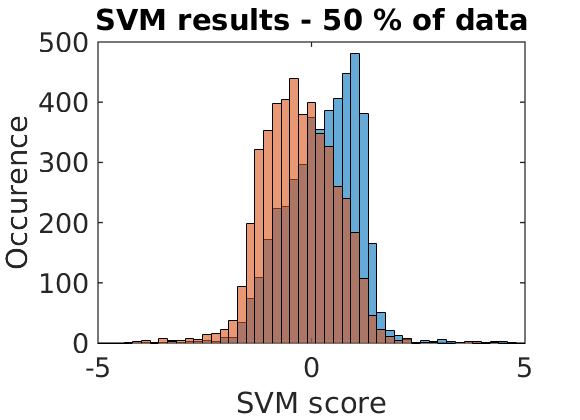
\includegraphics[width=\textwidth]{Pix/SVM_05_Score.png}
		\caption{Using 50\% of the data as training data.}
		\label{fig:SVM_05_score}
    \end{subfigure}
    \caption{The serperation of the two classes in terms of their SVM score. A value smaller (larger) than zero corresponds to the label "female" ("male")}
	\label{fig:SVM_Result}
\end{figure}
\FloatBarrier